\chapter{The effect of ions on unfolding force}
\label{sec:salt}

With the tools in place, it's time to do some science!  As a simple
experiment to demonstrate the utility of the new stack, I ran a series
of velocity clamp unfolding experiments on I27 octomers in PBS
(\cref{sec:sample-preparation}).  After a series of pulls in the
standard buffer, a buffer with additional calcium (from
\CaCl\citep{fisher-CaCl}) was flushed into the fluid cell.  After the
new buffer equilibrated, unfolding experiments were continued.

Since \citet{hofmeister88}, there has been a lot of research on the
effect of ions on protein solubility.  However, previous research on
the effect of ions on unfolding forces is small, but we do have some
material to work with.  Earlier experimental work on amyloid $\beta$
shows decreased fibrillation with even small
\Ca\ concentrations\citep{chauhan97,itkin11}.  The mechanism behind
this weaker bonding is unclear\citep{chauhan97,zhang06}, although
aspartic and glutamic acid groups tend to have a strong affinity for
cations while arginine has a strong affinity for the
\Cl\ anion\citep{friedman11}.  Of these amino acids, only glutamic
acid occurs in the key hydrogen bond regions responsible for I27
unfolding\citep{lu00b} (\cref{fig:I27:H-bonds}).  \NaCl\ has also been
shown to decrease internal hydrogen bonding in the
protein\citep{zidar11}.  In molecular dynamics studies of amalyoid
$\beta$ fragments, the destabilizing effect of \CaCl\ is much greater
than the destabilizing effects of \MgCl, \NaCl, and
\KCl\citep{smith13}.

\begin{figure}
  \begin{center}
    \includegraphics[width=0.5\textwidth]{figures/i27/1TIT-hbond}
    \caption{The backbone of I27 showing the eight key hydogen bonds
      responsible for the critical unfolding force.  Glutamic acids
      are highlighted in green.  Based on \xref{lu00b}{figure}{1b}.
      For a ribbon diagram of I27 showing the $\beta$-sheets, see
      \cref{fig:I27}.  This figure was also generated with
      \citetalias{pymol}.\label{fig:I27:H-bonds}}
  \end{center}
\end{figure}

We added $0.5\U{M}$ \CaCl\ to our standard PBS
(\cref{sec:sample-preparation}), which is much larger than
extracellular \Ca\ levels on the order of
$2\U{mM}$\citep{isaacs06,itkin11}.  After mixing, both buffers were
adjusted with drops of \HCl\ and \NaOH\ as needed to reach a pH around
7.5 (7.42 for the PBS, and 7.60 for the \Ca-enhanced PBS).

Unfolding experiments carried out on 2013-03-04 using our usual
procedure (\cref{sec:procedure}) yielded an unusual density of clean
unfolding curves\footnote{
  Experiments carried out using the same procedures throughout
  February were much less successful.
},
with 105 successful pulls concentrated in a two hour window.  Of these
pulls, 37 were in the standard PBS and 68 were in the enhanced
\Ca\ buffer.  Histograms of unfolding forces show decreased
unfolding forces in the \Ca\ buffer (\cref{fig:calcium:histogram}),
which is what we expect due to destabilized hydrogen bonding.

\begin{figure}
  \begin{center}
    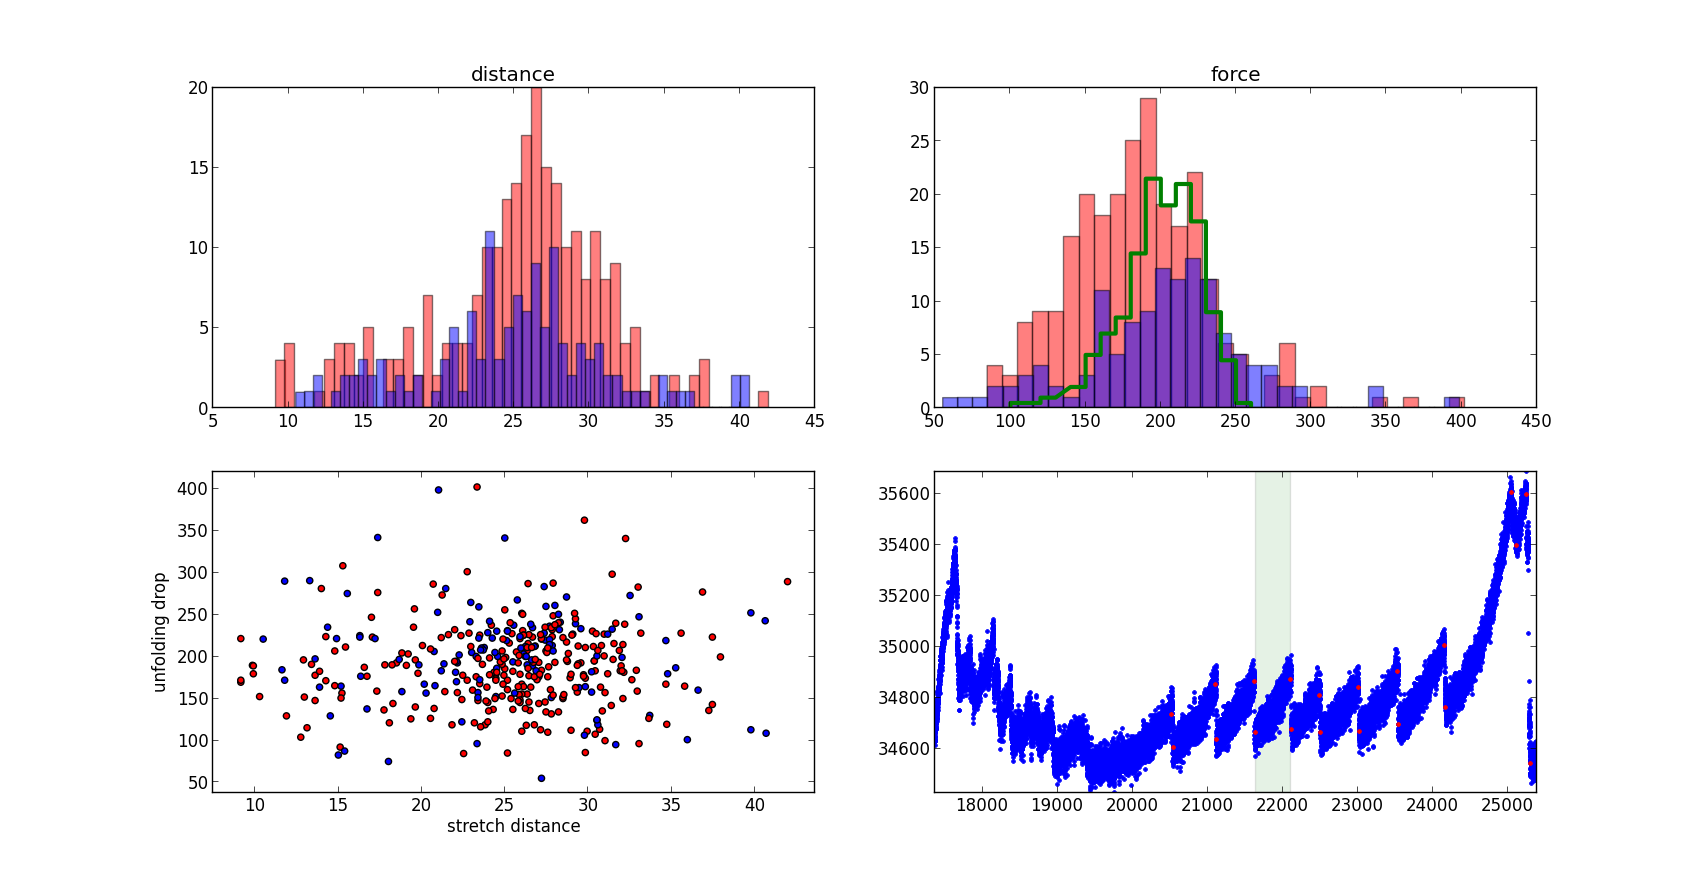
\includegraphics[width=0.9\textwidth]{figures/salt/2013-03-04-CaCl2}
    \caption{I27 runs from 2013-03-04 with (red) and without (blue) an
      extra $0.5\U{M}$ \Ca.  Clockwise from the upper left, we have
      the distance (in nm) between peaks, the unfolding force (in pN),
      and example force curve, and a scatter plot of unfolding force
      (in pN) versus the distance between peaks.  All of the pulls
      were taken with the same Olympus TR400-PSA cantilever with a
      pulling speed of $1\U{$\mu$m/s}$.  The green histogram drawn
      over the unfolding force histograms is I27 unfolding data in PBS
      with $5\U{mM}$ DTT from \citet{carrion-vazquez99b}, rescaled by
      a factor of $\frac{1}{2}$ because they had more unfolding
      events.\label{fig:calcium:histogram}}
  \end{center}
\end{figure}
%
\nomenclature[text ]{DTT}{Dithiothreitol
  (C\textsubscript{4}H\textsubscript{10}O\textsubscript{2}S\textsubscript{2}),
  also known as Cleland's reagent\citep{cleland64}.  It can be used to
  reduce disulfide bonding in proteins.}

Modeling I27 as a Bell-model unfolder, we can use \sawsim\ to find the
Bell parameters that best fit these experimental unfolding histograms
(\cref{sec:sawsim:rate:bell,sec:sawsim:results:fitting}).  The results
in \cref{fig:calcium:valley} show that the best fit for standard PBS
was with $\Delta x_u=0.132\U{nm}$ and $k_{u0}=0.222\U{s$^{-1}$}$.  In
the \Ca\ buffer, the best fit was with $\Delta x_u=0.123\U{nm}$ and
$k_{u0}=0.450\U{s$^{-1}$}$.

\begin{figure}
  \begin{center}
    \subfloat[][]{%
      \asyinclude{figures/salt/fit-valley-PBS}
      \label{fig:calcium:valley:pbs}}
    \subfloat[][]{%
      \asyinclude{figures/salt/fit-valley-PBS-0.5M-CaCl2}
      \label{fig:calcium:valley:pbs-calcium}}
    \caption{\protect\subref{fig:calcium:valley:pbs} Model fit quality
      for the standard PBS unfolding histogram data shown in
      \cref{fig:calcium:histogram}.
      \protect\subref{fig:calcium:valley:pbs-calcium} Model fit
      quality for the \Ca-enhanced PBS unfolding histogram data.  The
      best fit parameters occur when the Jensen--Shannon divergence is
      minimized (at the bottom of these valleys,
      \cref{sec:sawsim:results:fitting}).\label{fig:calcium:valley}}
  \end{center}
\end{figure}
